\documentclass[12pt]{article}
\usepackage[margin = .7in]{geometry}
\usepackage[USenglish]{babel}
\usepackage{natbib}
\usepackage{graphicx}
\usepackage{fancyhdr}
\usepackage{setspace}
\usepackage{amsmath}
\usepackage{lscape}
\usepackage{dcolumn}
\usepackage{xcolor}
\usepackage{longtable}
\usepackage[colorlinks=true,citecolor=red!50!black,urlcolor=blue!50!black,linkcolor=red!50!black]{hyperref}

\author{Laura Buchanan\footnote{\href{mailto:lcb402@nyu.edu}{lcb402@nyu.edu}} \and Patrick Kraft\footnote{\href{mailto:pk1622@nyu.edu}{pk1622@nyu.edu}}}
\date{today}

\title{Don't Just Ask Me for Facts!\\
\large{Measuring Political Sophistication using Open-Ended Responses}}
\date{\today}

% sans serif font
\renewcommand{\familydefault}{\sfdefault}


\begin{document}
\maketitle\doublespacing\thispagestyle{empty}

\begin{abstract}
There is a broad consensus among scholars of political science and public opinion that the American electorate is not well informed about politics. However, there is no agreement in the discipline about \textit{how to measure} how little citizens actually know. While many studies rely on simple factual political knowledge questions to assess political sophistication, others have criticized this approach from methodological and theoretical perspectives, claiming it does not provide a valid measure of the concept of interest. We propose a new measure of political sophistication based on open-ended survey responses about individual political attitudes and preferences. Using conventional political knowledge metrics and open-ended responses from the 2012 American National Election Study (ANES), we consider word count, topic diversity, opinion diversity, and a novel aggregate measure to show that text-based measures, while variable, capture aspects of sophistication unaccounted for when using conventional knowledge indices.  


\vspace{\baselineskip}
\noindent \textbf{Keywords:} political sophistication, measurement, open-ended responses, structural topic models \\

\noindent \textbf{Word Count:} $\sim$3,800
\end{abstract}
\newpage\setcounter{page}{1}



\section{Introduction}

One fundamental concept in the study of political attitudes and behavior is political sophistication and knowledge \citep{converse1964nature,carpini1996americans}. While most scholars emphasize how little people know about politics, how to assess individual knowledge has been subject to re-occurring scholarly debate \citep[e.g.][]{mondak2000reconsidering,mondak2001asked,sturgis2008experiment,debell2013harder,pietryka2013analysis}. Many analyses exclusively rely on individual levels of political knowledge measured by correctness of factual knowledge questions. However, recent research points to value in knowledge measures that have previously been disregarded 
\citep{barabas2014question}. Furthermore, scholars argue that factual political knowledge, as measured in many surveys, may not be theoretically relevant \citep{lupia2006elitism}. Rather, the political sophistication should take into account how people structure their attitudes and beliefs 
\citep[e.g.][]{luskin1987measuring}. As such, measuring sophistication solely based on answers to political trivia may misclassify respondents who cannot recall these facts, but do indeed have a coherent cognitive framework of political ideas.

We propose an alternative measure of political sophistication based on an individual's responses to open-ended political preference questions. We make inferences about the respondents' level of political sophistication and belief constraints by focusing on 
\textit{how} respondents describe their preferences and beliefs. We consider the diversity in topics raised by respondents. Topic diversity will be measured using structural topic models 
\citep{roberts2014structural}. Furthermore, we consider additional characteristics of open-ended responses, such as response length and diversity between opinions. Our aim is to assess how political attitudes are structured and expressed in a more complex manner than discernible from correctness on a factual questionnaire. We suspect that the diversity in topics a respondent discusses, or the topic detail with which they speak, will covary with other political knowledge measures. We therefore compare text-based measures to common factual knowledge measures. This text based analysis aims to be conceptually closer to the structure and constraint of political belief systems 
\citep[see for example][]{tetlock1983cognitive,luskin1987measuring} than fact based knowledge items can capture.
% revise last part depending on evaluation method etc.

Overall, we hope to show that our measure of political sophistication provides novel insights compared to conventional knowledge measures and provides new opportunities for comparisons of political knowledge across time and contexts.


\section{Political Knowledge and Sophistication}
% 1: defining political participation in the literature
% 2: measuring political sophistication, previous approaches
% 3: issues with previous approaches, criticism

In his seminal study, \citet{converse1964nature} examined how citizens hold constrained belief systems about politics. In the paper, belief systems are defined as ``a configuration of ideas and attitudes in which the elements are bound together by some form of constraint or functional interdependence'' \citep[207]{converse1964nature}. The analyses showed that the majority of the electorate does not hold structured and constrained belief systems, understand abstract ideological concepts, or hold stable issue positions. 

This pessimistic view regarding the competence of the US electorate has been supported in multiple subsequent analyses. \citet{carpini1996americans} show that large parts of the American electorate are not sufficiently informed about politics and there are systematic differences in political attitudes and behavior between citizens who are well informed compared to those who are not. These findings are problematic from a normative perspective, since they indicate that differences in political information can result in unequal representation in the political system \citep[see also][]{althaus1998information,kuklinski2000misinformation,gilens2001political}. However, rather than relying on the degree to which individuals hold constrained belief systems, \citet{carpini1996americans}, conceptualized knowledge as the awareness of key democratic values, using factual knowledge questions \citep[see also][]{carpini1993measuring}. Many studies focus on similar factual knowledge measures \citep[e.g.][]{zaller1991information,jacoby1995structure,gomez2001political}.  \citet{zaller1992nature} argued for the measurement of political awareness using tests of neutral factual information about politics, since they ``more directly than any of the alternative measures, capture what has actually gotten into people’s minds'' \citep[21]{zaller1992nature}. However, other research casts doubt on this assertion, both from methodological as well as theoretical perspectives.

Methodologically, many studies raised issues related to the validity of factual knowledge questions as a measure of political sophistication. One problem  are potential biases due to guessing \citep{mondak2000reconsidering,mondak2001developing,mondak2001asked,miller2008experimenting}. Knowledge items that offer a ``Don't Know'' option convolute two very distinct concepts: the individual information level and the propensity to guess. Based on this argument, \citet{mondak2004knowledge} show that conventional knowledge measures overestimate the gender gap in political knowledge due to male respondents being more likely to guess if they are not fully informed \citep[see also][]{pietryka2013analysis}. Their recommendation was to rely on closed rather than open-ended knowledge questions, and omitting ``Don't Know'' response options \citep[but see][]{sturgis2008experiment,luskin2011don}. Other scholars further criticized open-ended factual knowledge questions due to problematic coding rules, which do not capture partial knowledge \citep{krosnick2008problems,gibson2009knowing,debell2013harder}.

Focusing factual political knowledge has also been criticized on theoretical grounds. \citet{lupia2006elitism} argued that the information asked for in the item batteries has no clear relevance to political participation. Instead, researchers should concentrate on heuristics that directly help citizens to make competent political decisions \citep[see also][]{lupia1994shortcuts}. Responses to factual knowledge questions have further been shown to be conditional on the respondents' motivation, partisanship, and monetary incentives\citep{prior2008money,bullock2015partisan,prior2015you}. Conventional items also differ with regard to the dimension of political knowledge they measure \citep{barabas2014question} and ignore the import of aspects such as visual cues \citep{prior2014visual}.

Overall, the studies discussed suggest that the conventional item batteries have problematic measurement properties. More importantly, some authors raise doubts whether factual political knowledge actually captures the phenomena of interest. \citet{converse1964nature} focused on the level of constraint in political beliefs rather than isolated pieces of factual information. Other scholars, \citet{tetlock1983cognitive}, used \textit{integrative complexity} to describe the integration of considerations related to an issue. It is important to note that here, sophistication is not based on the content (or accuracy) of related considerations but rather on its \textit{structure}. \citet{luskin1987measuring} also defined political sophistication based on the structure of individual belief systems, arguing that belief systems can vary on three separate dimensions: (1) their \textit{size} -- i.e. the number of cognitions, (2) their \textit{range} -- i.e. the dispersion of cognition over categories, and (3) their \textit{constraint} -- i.e. the extent to which cognitions are interconnected. Political sophistication, in turn, is seen as the conjunction of these dimensions: ``A person is politically sophisticated to the extent to which his or her [political belief system] is large, wide-ranging, and highly constrained.'' \citep[860]{luskin1987measuring}.

Such a conceptualization of political sophistication seems theoretically useful than simple tests of factual information. Why does a large body of literature in political science and public opinion focus only on knowledge questions? One answer to this question is provided in the early study by \citet[206]{converse1964nature}, stating: ``what is important to study cannot be measured and that what can be measured is not important to study.'' Factual political knowledge is much easier to assess (albeit not perfectly) than the structure of political belief systems. Indeed, \citet{tetlock1983cognitive} had to rely on manual coding of policy statements of US senators to assess their degree of integrative complexity. Manual coding procedures, however, become infeasible with large text datasets (such as in large surveys). Advances in automated text analyses, provide us with the necessary tools to develop a measure of political sophistication that captures the theoretical arguments put forward by \citet{converse1964nature}, \citet{tetlock1983cognitive} and \citet{luskin1987measuring}, without human coders. In the following, we derive and explore a measure acting on open-ended survey responses.


\section{Measurement Approach}
% 1: describe measure and how it relates to theoretical conceptualization of sophistication (see Luskin's definition)
% 2: how are open-ended responses administered, potential issues
% 3: conclusion: coding open-ended responses gets us closer to the definition of political sophistication that we are actually interested in!

We propose that the dimensions laid out by \citet{luskin1987measuring} --- size, range, and constraint of political belief systems --- can be measured directly by examining how individuals describe their political attitudes and beliefs. More specifically, we consider individual responses to open-ended questions where respondents described aspects that they liked and disliked about both major political parties and presidential candidates before the 2012 US election. There are a total number of 8 open-ended responses where individuals describe their beliefs and attitudes towards political actors. Table~\ref{tab:measure} summarizes how different characteristics of open-ended responses match aspects of political sophistication discussed previously.

\begin{table}[h]
\begin{tabular}{ll}
\hline 
Dimension of political belief system & Characteristic of open-ended response \\
\hline
Size (number of cognitions) & Overall length of responses \\
Range (dispersion of cognitions over categories) & Diversity in topics raised in responses \\
Constraint (interconnectedness of cognitions) & Diversity in response length between items \\
\hline
\end{tabular}
\caption{Aspects of political sophistication and its measure in open-ended responses.}\label{tab:measure}
\end{table}

The size of the political belief system can be captured as the overall length of individual responses. If people possess a larger number of considerations related to political parties and candidates, then this should be reflected in the  overall collection of their responses.

The range of cognitions over categories can be measured as the diversity in topics raised in individual responses. If individuals hold more diverse cognitions towards political actors, we expect to observe a wider range of topics in their responses.

The last dimension, the degree of constraint or interconnectedness of cognitions, is more difficult to capture. While we cannot directly measure the interconnectedness of cognitions, we argue that the diversity in response length between items could be used as a possible proxy. Consider two individuals who possess a belief system of similar size and range. We expect that their open-ended responses should be of similar overall length and have a comparable degree of diversity in topics. Now, suppose that for one individual, the belief system is highly interconnected, and for the other individual it is not. Holding the overall length and topic diversity of their set of responses constant, higher interconnectedness allows homogeneous spread of topics across items. In other words, if considerations were not interconnected, then responding to likes and dislikes (for party/candidates of in/out-party), would require an increase in the overall length and diversity of the response. As such, distributing responses across different items indicates a higher diversity in opinions and can therefore be seen as a proxy for interconnectedness of cognitions.

Of course, the measurement strategy derived here makes strong implicit assumptions about the nature of political belief systems. However, the purpose of this discussion is to suggest potential links between the theoretical construct and measurable characteristics of open-ended responses. Ultimately it is an empirical question whether these characteristics provide valid measures of political sophistication. Before we turn to the issue of validation, we discuss the data and methods used in the analyses.



\section{Data and Methods}
% describe dataset and open-ended responses
% describe measure for each dimension as well as composite measure of sophistication

We use survey data from the 2012 American National Election Study (ANES) to demonstrate and validate our measures of political sophistication. The dataset consists of a survey of 5914 adults. 2054 participated in face-to-face interviews while the remaining 3860 participated online. While these samples differ slightly with regard to the inclusion of some variables, we rely on the pooled dataset purpose of our analysis.

Our sophistication measure acts on open-ended questions in which respondents were asked to list anything in particular that they like/dislike about the Democratic/Republican party as well as anything that might make them vote/not vote for either of the Presidential candidates. They were probed by the interviewer asking ``anything else?'' until the respondent answered no. Open-ended responses were pre-processed using an implementation of the Aspell spell checking algorithm in \texttt{R} (\url{www.aspell.net}), and dropping individuals who responded in Spanish (228 individuals). 

As discussed above, we consider three aspects of the open-ended responses to capture distinct dimensions of political sophistication: size, range, and constraint of the political belief system. The \textbf{size} of the belief system is measured as the word count for each individual over all prompts:
\begin{equation}
\text{size}_i = \log\left(\sum_{j=1}^J n_{ij}\right),
\end{equation}
where $n_{ij}$ is the number of words in the response of individual $i$ in response to question $j$. $J$ denotes the set of all likes/dislikes items. We use the log of the count normalize the distribution of responses. The \textbf{range} of the belief system is captured as the diversity in topics raised by each respondents. We conceptualize diversity as the Shannon-entropy of topic proportions \citep{shannon1948mathematical,munger2016elites}:\footnote{The structural topic model was estimated using the \texttt{stm} package in R \citep{roberts2014structural}. The number of topics was selected using the algorithm of \citet{lee2014low} and the model was estimated via spectral initialization to address the issue of multi-modality \citep[see][for details]{roberts2014stm}. We used measures for age, education, party identification, as well as an interaction between education and party identification as covariates for topic prevalence. This variable selection is equivalent to the procedure model specification described in \citet{roberts2014structural}. We estimated a total number of 72 topics. While we cannot discuss the topics in detail due to limited space, it is worth noting that the results reported hereafter are robust for model specifications with fewer numbers of topics.}
\begin{equation}
\text{range}_i = −\sum_{k=1}^K \theta_{ik} \log_2(\theta_{ik}),
\end{equation}
where $\theta_{ik}$ denotes the predicted proportion of topic $k$ in the collection of responses by individual $i$. The variable ranges from 0 (response focuses on single topic), to $\log_2(K=72)$ (every topic has the same proportion). As a proxy for \textbf{constraint}, we measure the diversity in opinions raised across item by computing the Shannon-entropy of the proportions of response lengths for each likes/dislikes question:
\begin{equation}
\text{constraint}_i = −\sum_{j=1}^J p_{ij} \log_2(p_{ij}),
\end{equation}
where $p_{ij}=\tfrac{n_{ij}}{\sum_{j=1}^J n_{ij}}$ is the proportion of words in the response of individual $i$ to question $j$ relative to the overall size of the individuals' response. Again, the variable ranges from 0 (only one question was answered) to $\log_2(J=8)$ (all questions were answered with the same word length per answer).

Together, the three measures form a composite metric of political sophistication. We combine the measures in a multiplicative rather than an additive fashion, because sophistication can be seen as \textit{conjunctive} \citep[see][]{luskin1987measuring}. In other words, the separate elements are only effective in combination and are not substitutes of each other:
\begin{equation}
\text{sophistication}_i = (\text{size}_i + 1) * (\text{range}_i + 1) * (\text{constraint}_i + 1).
\end{equation}
Note that we added $+1$ to each term to assure that the minimum of each individual variable is 1 rather than 0. This way, we still capture variation in sophistication if one of the elements is at its minimum.

We consider a number of conventional political knowledge measures for comparison with our metrics. The variables are summarized in Table~\ref{tab:featextr}. The first three measures are based on additive scales indicating the number of correct responses. The interviewer evaluation (only available in face-to-face sample) is based on a five-point scale that was recorded after the interviews (pre-election and post-election wave).

\begin{table}[h]\onehalfspacing\footnotesize
\begin{tabular}{p{5.5cm}p{5.5cm}p{5.5cm}}
\hline
Canonical Political Knowledge Metric &	Abridged Sample Questions &	Name in Figures \\
\hline
Knowledge of Office Recognition  	  & Who is the Speaker of the House? Who is the Vice President? &  Political Knowledge: Office Recognition \\ 
Knowledge of U.S. Political Facts 	 & How many times can someone be elected president? What is the size of the federal deficit? & Political Knowledge: Factual Knowledge\\
Knowledge of Majorities in Congress & What party has the most members in the U.S Senate? & Political Knowledge: Majorities in Congress\\
Pre-Interview Political Knowledge Interviewer Evaluation & --- & Political Knowledge: Knowledge Pre Evaluation\\
Post-Interview Political Knowledge Interviewer Evaluation & --- & Political Knowledge: Knowledge Pre Evaluation\\
Pre-Interview Intelligence Interviewer Evaluation & --- & Political Knowledge: Intelligence Pre Evaluation\\
Post-Interview Intelligence Interviewer Evaluation & --- & Political Knowledge: Intelligence Pre Evaluation\\
Education Level 	 & (1) Less than high school credential&Political Knowledge: Education Level \\
&(2) High School credential&\\
&...&\\
&(5) Graduate School & \\
\hline 
\end{tabular} 
\caption{Methods: Feature Extraction}\label{tab:featextr}
\end{table}

Furthermore, the analyses outlined below includes several control variables such as media exposure, frequency of political discussions, gender, age, race, religiosity, ideology, party identification, and survey mode (face-to-face vs. online).
	

\section{Descriptive Results}
% histogram of response length could be useful -> done
% histogram of individual aspects -> done
% show examples of high and low scoring political knowledge -> appendix
% distribution of knowledge measure -> done
% correlation plot with other knowledge measures (including individual aspects) -> done

First, we examine the characteristics of open-ended responses as a measure of political sophistication. Figure~\ref{fig:wc} displays the word count as well as the logged word count of the collection of open-ended responses for each individual.

\begin{figure}[h]
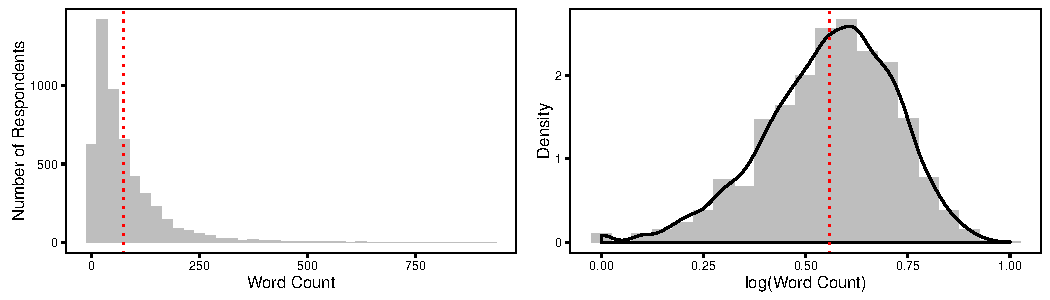
\includegraphics[width=\textwidth]{../fig/wc.pdf}
\caption{Distribution of Response Lengths}\label{fig:wc}
\end{figure}

The distribution of raw word count is highly skewed. Most respondents provide brief statements when they describe their attitudes towards political parties and candidates. The mean response length to all 8 questions is about 75 words, so an average response to a single question consisted of less than 10 words, omitting respondents who did not provide any information.
\begin{figure}[h]
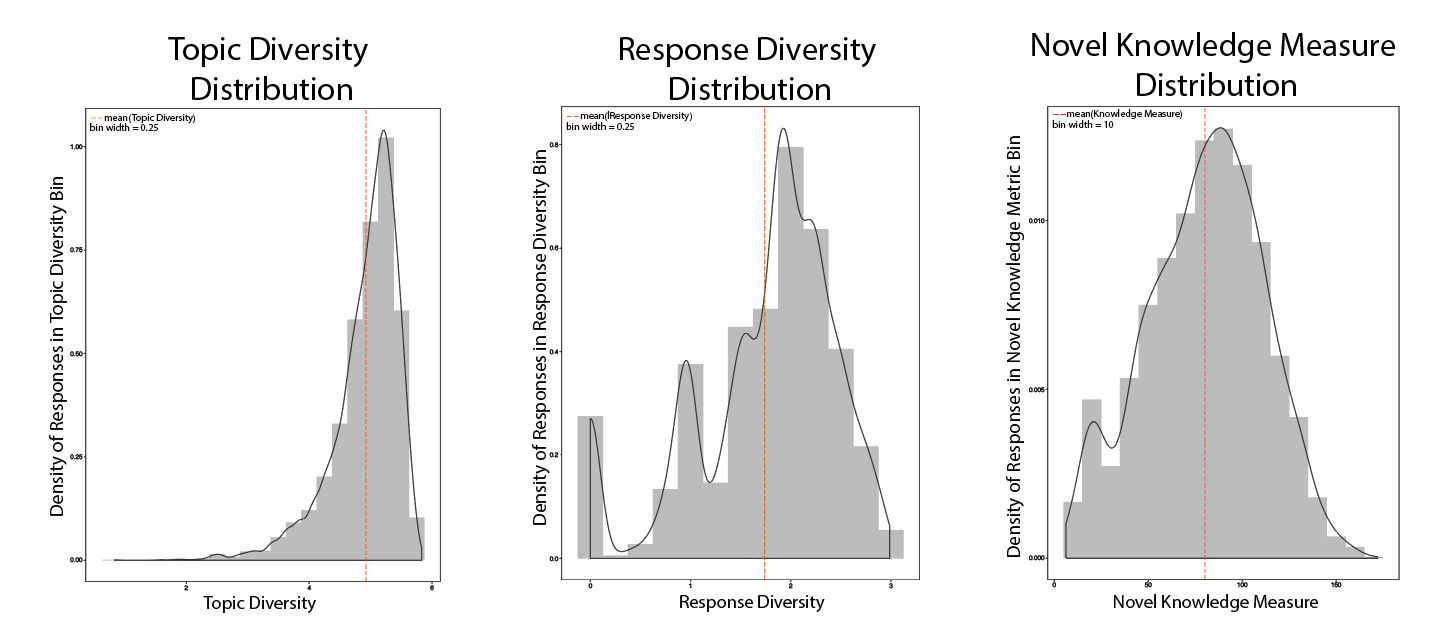
\includegraphics[width=\textwidth]{../fig/diversity_distributions.png}
\caption{Diversity Distributions and Sophistication Measure}\label{fig:diversity}
\end{figure}

Figure~\ref{fig:diversity} presents histograms of the remaining two diversity measures as well as the composite index of political sophistication. Diversity across topics (left panel) is skewed and overall relatively large. Only few respondents appeared to focus on a very select number of topics. As we discuss below, this finding can be partly attributed to the way topic proportions are estimated in the structural topic model. The distribution of response diversity (or opinion/item diversity, see middle panel), on the other hand, indicates that a large proportion of respondents only answered one open-ended question, which leads to a response diversity of 0. Looking at the histogram on the right in Figure~\ref{fig:diversity}, we can see that the combined measure of sophistication is approximately normal and captures a large amount of variance between individuals. But is this variance also conceptually meaningful?


\section{Validation Performance}
% replicate common findings, e.g. gender gap in political knowledge \citep[e.g.][]{barabas2014question}
% Increase in consistency b/w policy attitudes \citep[e.g.][]{prior2014visual}

First, we examine the face validity of the measure. In the appendix, we show examples of survey responses and their estimated sophistication value. The first table displays responses with the minimum and maximum composite score in the dataset.  Short responses are clearly penalized. The second table shows the responses with minimum and maximum composite scores for a subset of the data where the response was between 50 and 100 words. We see that the score is not only based on word length, but also topic diversity and diversity across items. This initial investigation suggests that the variation in the sophistication measure captures interesting differences in response behavior.

Next, we compare our measure with conventional knowledge indices. Figure~\ref{fig:corr} displays a correlation matrix of the traditional measures as well as the individual open-ended response characteristics and the composite measure of sophistication.

\begin{figure}[h]
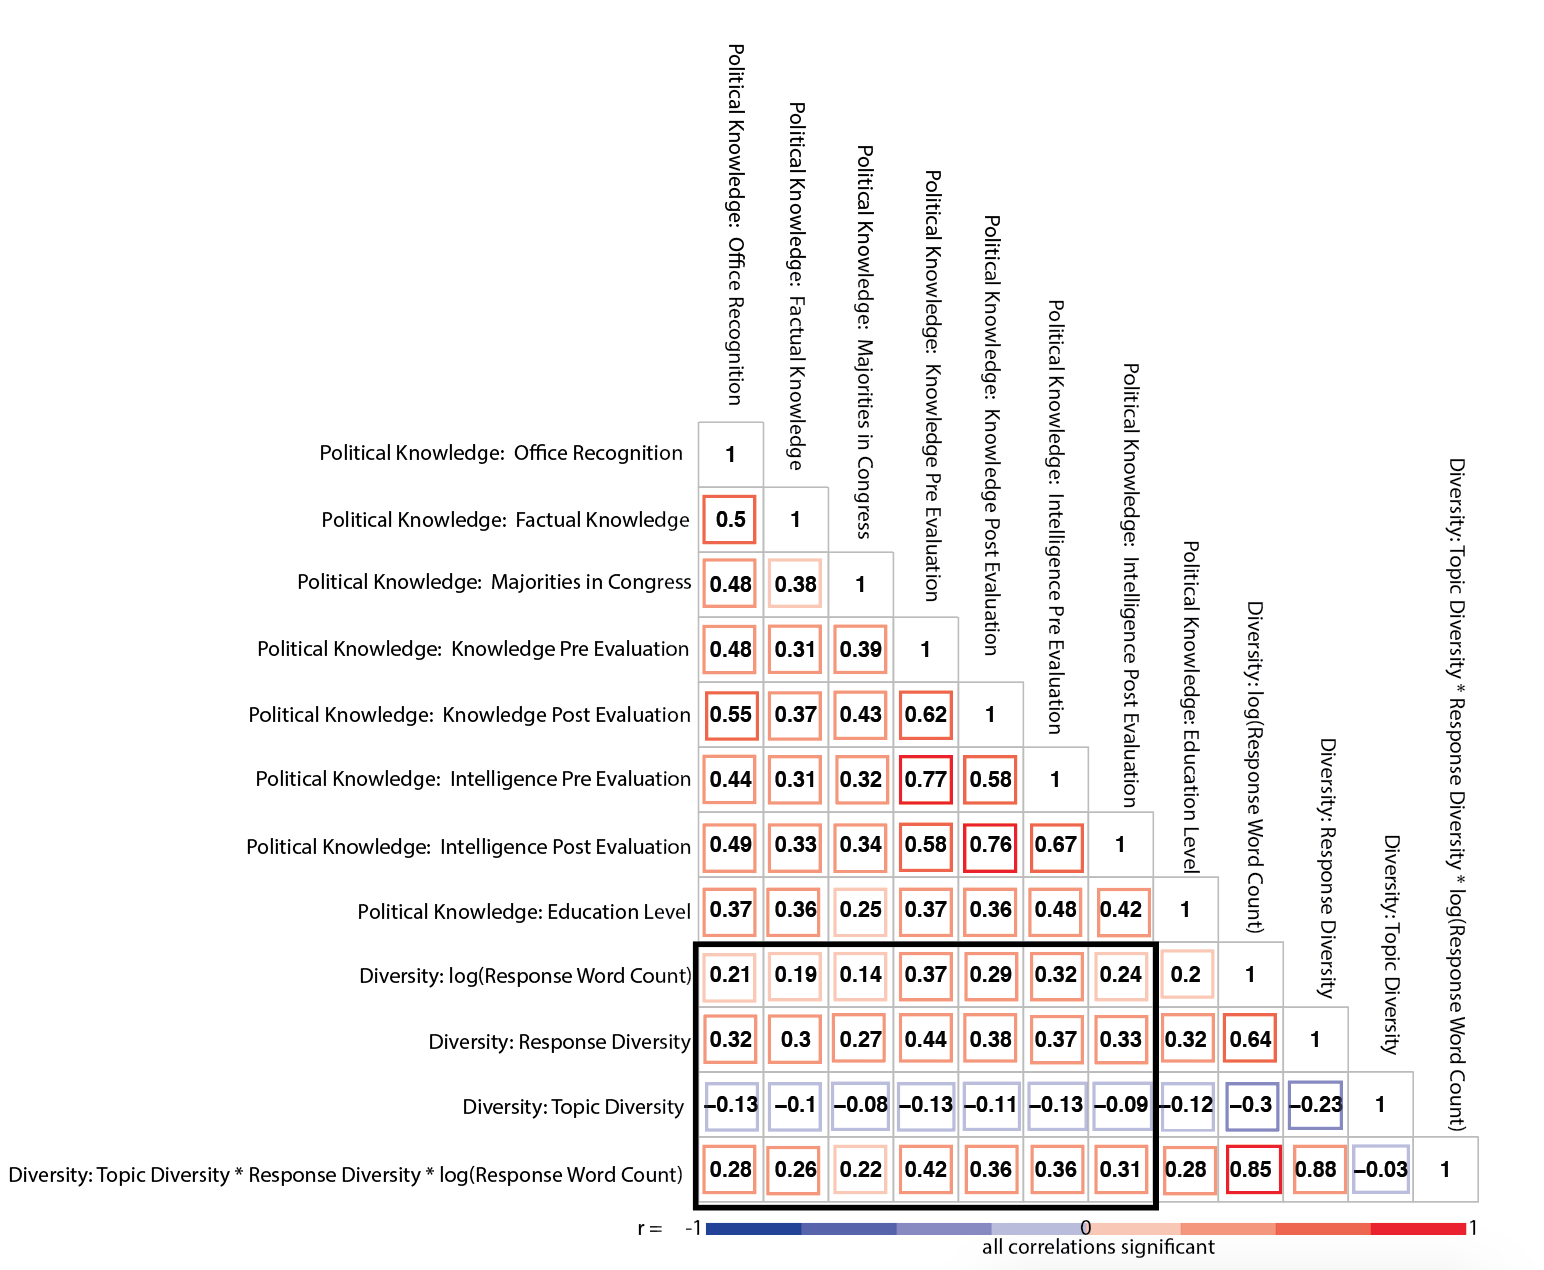
\includegraphics[width=\textwidth]{../fig/corr_fixed_data.png}
\caption{Correlation Plot of Knowledge Measures}\label{fig:corr}
\end{figure}

The bold black box highlights the correlations between the political knowledge measures and the open-ended response measures.  Our first observation is that political knowledge measures are modestly to strongly correlated with one another.  This finding is interesting; while it confirms that these measures do covary to some degree, they are not all capturing the same types of knowledge, as might be expected.  Next, we see that Topic Diversity has low negative correlation with all other measures.  This suggests that topic diversity alone, in this context, is not an appropriate measure of political knowledge.  A possible explanation for this finding is that the posterior topic proportions of the structural topic model are not only determined by the words in each response but also the respective prior over topics. As such, if a respondent only mentions a single word in his or her response, the estimated topic proportions will be still be relatively equal (i.e. indicating high diversity), rather than strictly unitary. Therefore, short responses may overestimate topic diversity with our method, explaining negative correlations with traditional knowledge measures. However, we leave this issue for further extensions and note that any potential biases caused by this issue are (at least partly) compensated by including overall response lengths and opinion diversity in the resulting sophistication measure.

We also see the Response Diversity and the composite final diversity metric have stronger correlations with the political knowledge measures than log(Response Word Count), suggesting that these two diversity measures are not strictly due to the length of the open-ended responses.  Finally, our final composite diversity score correlates across other political knowledge measures on the same order of magnitude as Factual Knowledge and Majorities in Congress, yet do not have especially high correlation with either.  This is evidence that our composite diversity score is worthy of consideration among standard political knowledge measures, and captures independent information.    

\begin{figure}[h]
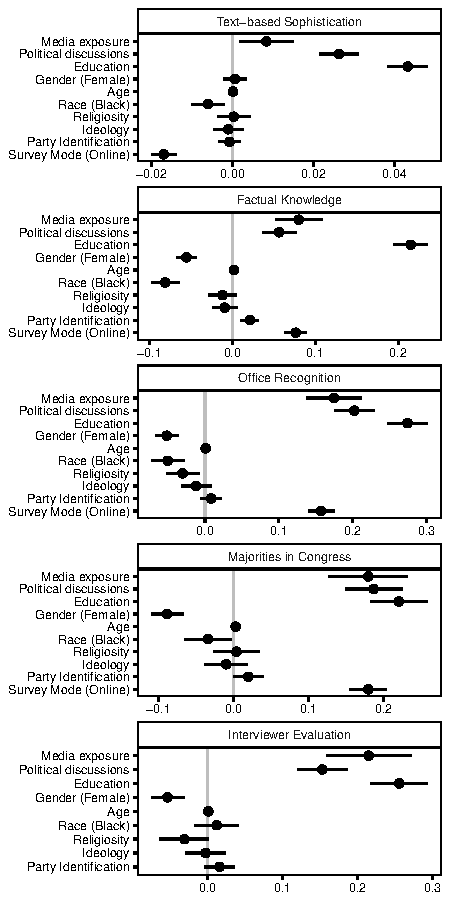
\includegraphics[width=\textwidth]{../fig/models.pdf}
\caption{Comparing Determinants of Political Sophistication}\label{fig:models}
\end{figure}

The next step of out validation consists of comparing the results for common determinants of political knowledge across the conventional as well as our text-based measure of political sophistication. Previous studies consistently showed that political knowledge is positively affected by media exposure, frequent political discussions, and education. Furthermore, research frequently finds a gender gap, where female respondents appear to be less informed about politics \citep[c.f.][]{barabas2014question}.\footnote{However, as discussed previously, this gap can be partly attributed to differences in the propensity to guess in factual knowledge questions \citep[e.g.][]{mondak2004knowledge}.} Figure~\ref{fig:models} displays the coefficients of regression models with each knowledge/sophistication measure as the dependent variable.

Overall, the patterns are quite similar across different dependent variables. Knowledge and sophistication is significantly higher among respondents who are more exposed to political news media, discuss politics frequently, and are more educated. However, there are some noteworthy and interesting differences between the conventional indices and our text-based measure. Most importantly, while we observe the common gender gap using factual knowledge questions and interviewer assessments, this difference disappears when looking at sophistication based on open-ended responses. Women might not score as high on political information quizzes (partly because they are less likely to guess rather express lack of knowledge), but they do not differ substantially in complexity and sophistication when they describe their political preferences. Another interesting finding is the effect of survey mode. For factual knowledge questions, we observe that respondents in online surveys score significantly higher than individuals in face-to-face interviews. This difference could be explained by the fact that individuals are able to look up responses to factual knowledge questions while taking an online survey. For the text-based measure, on the other hand, we see that individuals appear to score lower on sophistication in online surveys. Respondents in online surveys might therefore be less willing to elaborate on their attitudes.


\section{Conclusion}
% lot's of potential extensions, think about standardizing the measure to make it more comparable across contexts

Previous research in political science and public opinion has raised multiple theoretical and methodological issues related to conventional political knowledge indices. The goal of this paper is to examine an alternative measure of political sophistication based on open-ended responses in surveys. It was argued that this measure is conceptually closer to theoretical approaches that emphasize the importance of the structure and complexity of belief systems rather than focusing on factual knowledge about institutions. Overall, our findings show that conventional knowledge indices and the text-based measure share a substantial amount of variance. However, they are far from being identical and capture different aspects of sophistication. One of the most interesting findings is that using the text-based measure, we don't find evidence for a gender gap that has been commonly reported using factual knowledge scales. While further work on validation and the comparability of the measure across contexts and survey modes seems necessary, we think that measuring political sophistication based on open-ended responses has the potential to provide novel insights into the antecedents and consequences of political information.

\clearpage\singlespacing\footnotesize
\bibliographystyle{apsr2006}
\bibliography{lit}

\clearpage
\section*{Appendix: Samples of Open-Ended Responses for High/Low Sophistication}

% latex table generated in R 3.3.0 by xtable 1.8-2 package
% Wed May 11 10:13:17 2016
\begin{longtable}[ht]{p{1.4cm}lp{12cm}}
  \hline
 & Minimum & Maximum \\ 
  \hline
Case ID & 4258 & 1905 \\ 
  Obama (likes) & -1 Inapplicable & He's more likely to continue to support biomedical research as president, I think he's stronger on domestic issues, funding domestic programs, less likely to be influenced by corporate lobby, as President has shown not to be, less likely to make poor decisions regarding our occupation of other countries which we can ill afford, he'd be inclined to support education and infrastructure and more likely to support seeking alternative energy sources \\ 
  Obama (dislikes) & -1 Inapplicable & I don't think that he is a realist with regards to the terrorist threats, he's attempted to be too diplomatic with his foreign policy with regard to terrorism and terrorist threats, He's a very good politician and that's sort of a detriment, his 1st termhe tried too much to work 'across the aisle' and didn't realize the how steadfast and polarized the opposition was, I would like to see more strength in his resolve of his views, he was too willing to compromise his beliefs to get things done, I don't necessarily agree with the way he's handling his support of Israel, could be more openly supportive than he is \\ 
  Romney (likes) & -1 Inapplicable & He has consistently been openly supportive of Israel and the Israeli state.  Israel is right to exist in that region.  I believe that his experience in economics and investment probably did prepare him to be an efficient leader and someone who knows a lot about economic policy. He seems like a nice family man, politically I can't think of a lot more than that. \\ 
  Romney (dislikes) & -1 Inapplicable & I don't trust him at all. I think he's an out of touch wealthy politician who would say anything to get elected and has been caught on tape essentially admitting in so many words that he is a racist. He chose Paul Ryan as a running mate, that decision inand of itself was enough to make me know I don't want to vote for him. He fundamentally believes that more than 50 percent  percent of this country are shiftless layabouts who aren't interested in working.  That's obviously the view of someone whose mind is out of touch with what's going on in this country. He's a misogynist. \\ 
  Democratic party (likes) & Compassion & They generally are supportive of domestic spending, specifically on research and technology, and education. They tend to lean toward a more reserved approach to foreign policy, less aggressive, they tend to be people who are more emphathetic and care fortheir fellow man, which is mostly good \\ 
  Democratic party (dislikes) & -1 Inapplicable & They tend to be faster to raise taxes. They have a tendency toward extreme idealism.  That can be dangerous because not everyone wants to be or can be saved by entitlement programs. \\ 
  Republican party (likes) & -1 Inapplicable & They have adopted this systematic approach towards the support of Israel. Their logic and reason behind it are poor, but I agree with the suppost. Fiscal conservatism, in theory, is a good thing. It's good to make smart decisions about spending and not frivilously spend money.  The stance to support small businesses is encouraging, but a disingenuous party platform. \\ 
  Republican party (dislikes) & -1 Inapplicable & I think the modern Republican party has been hijacked by Christian conservatives who set policy based on their religious beliefs.  In addition, a wave of back lash political support in opposition to Obama spawned this tea party movement, which is just ananti-entitlement, anti-gay, pro-guns and God grassroots campaign that has taken over. \\ 
   \hline
   \caption{Example of open-ended responses for minimum and maximum score of political sophistication measure (among all responses). Note that these are the raw responses without any pre-processing (such as spell-checking, removal of terms like ``-1 Inapplicable'', removal of punctuation, stemming, etc.),}
\end{longtable}

\newpage
% latex table generated in R 3.3.0 by xtable 1.8-2 package
% Wed May 11 10:25:59 2016
\begin{longtable}[ht]{p{4cm}p{6cm}p{6cm}}
   \hline
  & Minimum & Maximum \\ 
   \hline
 Case ID & 3093 & 4115 \\ 
   Obama (likes) & -1 Inapplicable & i think he has done well so far \\ 
   Obama (dislikes) & Shady. He left his spot in Illinois and someone is in prison for trying to sell it. Wonder how he got it. Probably the same way he got the Nobel. Who's in charger of USDA school program? Who is surgeon General? How they get there? What are their true credentials prior to current positions? Reeks. & way things are going with education \\ 
   Romney (likes) & -1 Inapplicable & his health policy outlooks, but it also hinders itself as well. his pro-life opinion \\ 
   Romney (dislikes) & -1 Inapplicable & personality a lot of his policies \\ 
   Democratic party (likes) & -1 Inapplicable & i like their ideas they are for the people \\ 
   Democratic party (dislikes) & They care about the stupidest stuff & sometimes i wonder if progress can occur \\ 
   Republican party (likes) & -1 Inapplicable & my religous beliefs of Christianity tend to follow many of their thoughts \\ 
   Republican party (dislikes) & Stewards for the rich and big business & soemtimes they don't make sense or have just never been 'the right mix' to make me want to vote for them \\ 
    \hline
  \caption{Example of open-ended responses for minimum and maximum score of political sophistication measure (only responses between total length of 50 and 100 words). Note that these are the raw responses without any pre-processing (such as spell-checking, removal of terms like ``-1 Inapplicable'', removal of punctuation, stemming, etc.).}
  \label{tab:ex1}
\end{longtable}

\end{document}